% Figura: exemplo do PSP (instância A/0020, Solução C) — gerada em TikZ
\documentclass[tikz,border=4pt]{standalone}
\usepackage[utf8]{inputenc}
\usepackage[T1]{fontenc}
\usepackage{times}
\usepackage{amsmath}
\usetikzlibrary{shapes.geometric}
\tikzset{
  caixa/.style={draw=black!70, line width=0.5pt, fill=white},
  sel/.style={draw=green!45!black, line width=1.4pt, fill=green!5},
  piso/.style={draw=black!60, line width=0.5pt},
  rotulo/.style={font=\small},
  titulo/.style={font=\normalsize},
}
% Item 0: círculo | Item 1: triângulo | Item 2: losango | Item 3: estrela | Item 4: cilindro
\newcommand{\shpa}[1]{\fill[blue!20,draw=blue!55] #1 circle (0.12);}
\newcommand{\shpb}[1]{\node[regular polygon,regular polygon sides=3,minimum size=0.34cm,inner sep=0pt,fill=red!25,draw=red!60] at #1 {};}
\newcommand{\shpc}[1]{\node[diamond,minimum size=0.30cm,inner sep=0pt,fill=yellow!40,draw=orange!70] at #1 {};}
\newcommand{\shpd}[1]{\node[star,star points=5,star point ratio=2.2,minimum size=0.32cm,inner sep=0pt,fill=violet!25,draw=violet!60] at #1 {};}
\newcommand{\shpe}[1]{\begin{scope}[shift={#1}]
  \filldraw[fill=green!25,draw=green!50!black] (-0.1,0.09) -- (-0.1,-0.09) arc[start angle=180,end angle=360,x radius=0.1,y radius=0.045] -- (0.1,0.09);
  \filldraw[fill=green!15,draw=green!50!black] (0,0.09) ellipse[x radius=0.1,y radius=0.045];
\end{scope}}
\begin{document}
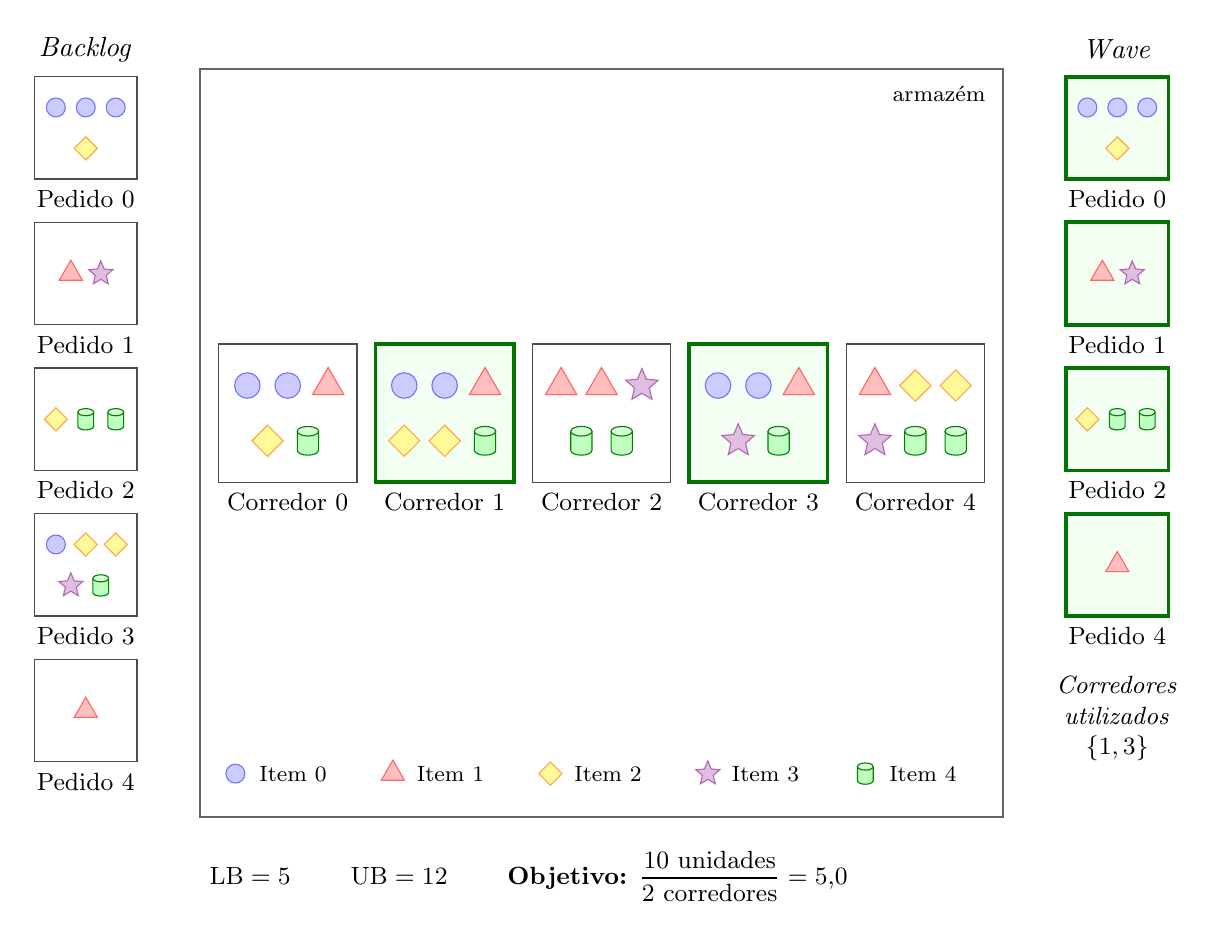
\begin{tikzpicture}
\node[titulo] at (0.65,10.25) {\textit{Backlog}};
\begin{scope}[shift={(0,8.6)},scale=1.0,transform shape]
\draw[caixa] (0,0) rectangle ++(1.3,1.3);
\shpa{(0.270,0.910)}
\shpa{(0.650,0.910)}
\shpa{(1.030,0.910)}
\shpc{(0.650,0.390)}
\end{scope}
\node[rotulo] at (0.65,8.35) {Pedido 0};
\begin{scope}[shift={(0,6.75)},scale=1.0,transform shape]
\draw[caixa] (0,0) rectangle ++(1.3,1.3);
\shpb{(0.460,0.650)}
\shpd{(0.840,0.650)}
\end{scope}
\node[rotulo] at (0.65,6.5) {Pedido 1};
\begin{scope}[shift={(0,4.8999999999999995)},scale=1.0,transform shape]
\draw[caixa] (0,0) rectangle ++(1.3,1.3);
\shpc{(0.270,0.650)}
\shpe{(0.650,0.650)}
\shpe{(1.030,0.650)}
\end{scope}
\node[rotulo] at (0.65,4.6499999999999995) {Pedido 2};
\begin{scope}[shift={(0,3.049999999999999)},scale=1.0,transform shape]
\draw[caixa] (0,0) rectangle ++(1.3,1.3);
\shpa{(0.270,0.910)}
\shpc{(0.650,0.910)}
\shpc{(1.030,0.910)}
\shpd{(0.460,0.390)}
\shpe{(0.840,0.390)}
\end{scope}
\node[rotulo] at (0.65,2.799999999999999) {Pedido 3};
\begin{scope}[shift={(0,1.1999999999999993)},scale=1.0,transform shape]
\draw[caixa] (0,0) rectangle ++(1.3,1.3);
\shpb{(0.650,0.650)}
\end{scope}
\node[rotulo] at (0.65,0.9499999999999993) {Pedido 4};
\draw[piso] (2.1,0.49999999999999933) rectangle (12.3,10.0);
\node[anchor=north east,font=\footnotesize] at (12.200000000000001,9.9) {armazém};
\begin{scope}[shift={(2.3375000000000004,4.749999999999999)},scale=1.35,transform shape]
\draw[caixa] (0,0) rectangle ++(1.3,1.3);
\shpa{(0.270,0.910)}
\shpa{(0.650,0.910)}
\shpb{(1.030,0.910)}
\shpc{(0.460,0.390)}
\shpe{(0.840,0.390)}
\end{scope}
\node[rotulo] at (3.2150000000000003,4.499999999999999) {Corredor 0};
\begin{scope}[shift={(4.33,4.749999999999999)},scale=1.35,transform shape]
\draw[caixa,sel] (0,0) rectangle ++(1.3,1.3);
\shpa{(0.270,0.910)}
\shpa{(0.650,0.910)}
\shpb{(1.030,0.910)}
\shpc{(0.270,0.390)}
\shpc{(0.650,0.390)}
\shpe{(1.030,0.390)}
\end{scope}
\node[rotulo] at (5.2075000000000005,4.499999999999999) {Corredor 1};
\begin{scope}[shift={(6.322500000000001,4.749999999999999)},scale=1.35,transform shape]
\draw[caixa] (0,0) rectangle ++(1.3,1.3);
\shpb{(0.270,0.910)}
\shpb{(0.650,0.910)}
\shpd{(1.030,0.910)}
\shpe{(0.460,0.390)}
\shpe{(0.840,0.390)}
\end{scope}
\node[rotulo] at (7.200000000000001,4.499999999999999) {Corredor 2};
\begin{scope}[shift={(8.315000000000001,4.749999999999999)},scale=1.35,transform shape]
\draw[caixa,sel] (0,0) rectangle ++(1.3,1.3);
\shpa{(0.270,0.910)}
\shpa{(0.650,0.910)}
\shpb{(1.030,0.910)}
\shpd{(0.460,0.390)}
\shpe{(0.840,0.390)}
\end{scope}
\node[rotulo] at (9.1925,4.499999999999999) {Corredor 3};
\begin{scope}[shift={(10.307500000000001,4.749999999999999)},scale=1.35,transform shape]
\draw[caixa] (0,0) rectangle ++(1.3,1.3);
\shpb{(0.270,0.910)}
\shpc{(0.650,0.910)}
\shpc{(1.030,0.910)}
\shpd{(0.270,0.390)}
\shpe{(0.650,0.390)}
\shpe{(1.030,0.390)}
\end{scope}
\node[rotulo] at (11.185,4.499999999999999) {Corredor 4};
\shpa{(2.5500000000000003,1.0499999999999994)}
\node[anchor=west,font=\footnotesize] at (2.7300000000000004,1.0499999999999994) {Item 0};
\shpb{(4.550000000000001,1.0499999999999994)}
\node[anchor=west,font=\footnotesize] at (4.73,1.0499999999999994) {Item 1};
\shpc{(6.550000000000001,1.0499999999999994)}
\node[anchor=west,font=\footnotesize] at (6.73,1.0499999999999994) {Item 2};
\shpd{(8.55,1.0499999999999994)}
\node[anchor=west,font=\footnotesize] at (8.73,1.0499999999999994) {Item 3};
\shpe{(10.55,1.0499999999999994)}
\node[anchor=west,font=\footnotesize] at (10.73,1.0499999999999994) {Item 4};
\node[titulo] at (13.750000000000002,10.25) {\textit{Wave}};
\begin{scope}[shift={(13.100000000000001,8.6)},scale=1.0,transform shape]
\draw[caixa,sel] (0,0) rectangle ++(1.3,1.3);
\shpa{(0.270,0.910)}
\shpa{(0.650,0.910)}
\shpa{(1.030,0.910)}
\shpc{(0.650,0.390)}
\end{scope}
\node[rotulo] at (13.750000000000002,8.35) {Pedido 0};
\begin{scope}[shift={(13.100000000000001,6.75)},scale=1.0,transform shape]
\draw[caixa,sel] (0,0) rectangle ++(1.3,1.3);
\shpb{(0.460,0.650)}
\shpd{(0.840,0.650)}
\end{scope}
\node[rotulo] at (13.750000000000002,6.5) {Pedido 1};
\begin{scope}[shift={(13.100000000000001,4.8999999999999995)},scale=1.0,transform shape]
\draw[caixa,sel] (0,0) rectangle ++(1.3,1.3);
\shpc{(0.270,0.650)}
\shpe{(0.650,0.650)}
\shpe{(1.030,0.650)}
\end{scope}
\node[rotulo] at (13.750000000000002,4.6499999999999995) {Pedido 2};
\begin{scope}[shift={(13.100000000000001,3.049999999999999)},scale=1.0,transform shape]
\draw[caixa,sel] (0,0) rectangle ++(1.3,1.3);
\shpb{(0.650,0.650)}
\end{scope}
\node[rotulo] at (13.750000000000002,2.799999999999999) {Pedido 4};
\node[align=center,font=\small] at (13.750000000000002,1.7499999999999993) {\textit{Corredores}\\\textit{utilizados}\\$\{1,3\}$};
\node[anchor=west,font=\small] at (2.1,-0.2500000000000007) {$\mathrm{LB} = 5$ \qquad $\mathrm{UB} = 12$ \qquad \textbf{Objetivo:} $\dfrac{\text{10 unidades}}{\text{2 corredores}} = 5{,}0$};
\end{tikzpicture}
\end{document}
